\pdfoutput=1
\documentclass[11pt]{article}
\usepackage[final]{acl}
\usepackage{times}
\usepackage{latexsym}
\usepackage[T1]{fontenc}
\usepackage[utf8]{inputenc}
\usepackage{microtype}
\usepackage{inconsolata}
\usepackage{graphicx}
\usepackage{booktabs}
\usepackage{multirow}
\usepackage{amsmath}

\newcommand{\x}{$\times$}

\title{Removing the Token Tax from an Existing Model:\\A Vocabulary Extension for 24 Indian Languages\\That Keeps Every Other Token}

\author{Sankur Kundu \\
  Independent researcher, Bhubaneswar, India \\
  \texttt{sankur.kundu.tw@gmail.com}}

\begin{document}
\maketitle

\begin{abstract}
The same sentence costs more tokens in an Indian language than in English, so Indian-language users
pay more per answer, wait longer for it and fit less text into a model's context. We measure this
token tax for the 24 Indian languages in FLORES-200 across 15 tokenizers that ship with current
models, and separate its two causes using the pre-tokenization bound of \citet{regmi2026vowel}. In
the GPT-4, Llama~3 and Qwen tokenizers the pre-tokenizer alone keeps Odia at no less than 2.32\x\
the tokens of English (Hindi 2.35\x, Tamil 2.64\x); Mistral's Tekken has no such bound (0.84\x\ for Odia) but
its vocabulary still costs 12.9\x\ English, and two Indian models, Krutrim-2 and Sarvam-M, ship it
unchanged. We then remove both causes from Qwen~2.5's tokenizer without changing a single
token id for English, code or any non-Indic script, by confining new merges to Indic byte prefixes
and relaxing the pre-tokenizer only for Indic combining marks. The result, lipi-Indic, uses fewer
tokens than the tokenizers of GPT-4o and Gemini in 23 of 24 languages (speaker-weighted 1.30\x\
English, against 1.92\x\ and 1.58\x) with a smaller vocabulary than Gemini's. On Qwen~2.5~0.5B, an
Odia version trains on the same text 5.4\x\ faster and, in equal GPU time, reaches 20\% lower bits
per byte on held-out Odia web text; generation is 2.3--7.0\x\ faster across Indian languages and
prefill of a 3,000-character Odia document 39\x\ faster. Along the way we find 1,667 tokens in
Qwen~2.5's vocabulary that its own pre-tokenizer can never produce and whose embeddings sit close to
the mean embedding, consistent with never having been trained. Code, tokenizers and all measurements
are released.\footnote{\url{https://github.com/Shakhtar-Sankur/lipi}}
\end{abstract}

\section{Introduction}

A language model reads, writes, is priced and is limited in tokens. When a tokenizer needs more
tokens for the same content in one language than another, speakers of the first pay more per
request, wait longer for every generated sentence and fit less of their text into the model's
context window \citep{petrov2023unfairness,ahia2023allcost}. For the languages of India, spoken by
more than a billion people, this \emph{token tax} is large and uneven. On GPT-4o's tokenizer the
FLORES-200 devtest \citep{nllb2022} costs 1.57\x\ the tokens of English in Hindi but 4.99\x\ in Odia,
spoken by 37.5 million people, and 13.7\x\ in Santali (Ol Chiki script).

Recent work has measured the tax for Indian languages \citep{srivastava2026tokenizertax}, argued
that pre-tokenization matters more than the subword algorithm for complex scripts
\citep{velayuthan2025egalitarian}, shown that a pre-tokenizer whose word class omits combining marks
imposes a lower bound on the token count of abugida scripts that no vocabulary can overcome
\citep{regmi2026vowel}, and proposed new Indic-capable tokenizers
\citep{shravan2026brahmic,rana2025mutant}. A new tokenizer, however, requires a new model or a costly
re-embedding of an existing one. This paper asks how much of the tax can be removed from a model that
already exists, without disturbing anything it knows, and makes the following contributions:

\begin{enumerate}
\item \textbf{The two causes, per current tokenizer and Indian language} (\S\ref{sec:measure}).
Computing the pre-tokenization bound of \citet{regmi2026vowel} (our \emph{floor}) for 15 current
tokenizers and all 24 Indian languages of FLORES-200 separates them: the GPT-4, Llama~3 and Qwen
pre-tokenizers alone impose 2.13--2.66\x\ English on the Brahmic scripts, while GPT-4o, Llama~4,
DeepSeek-V3 and Tekken have floors of 0.69--1.10\x\ on the same scripts and owe their tax to the
vocabulary. Krutrim-2
and Sarvam-M, two models built in India, ship Tekken unchanged, inheriting the highest Odia tax among
major tokenizers (12.9\x).
\item \textbf{An extension that keeps every other token} (\S\ref{sec:fix}). We remove both causes from
Qwen~2.5's tokenizer while leaving the token ids of English, code and every non-Indic language
identical, so the existing embeddings for them remain valid. lipi-Indic takes fewer tokens than
GPT-4o's and Gemini's tokenizers in 23 of 24 Indian languages.
\item \textbf{Unreachable tokens} (\S\ref{sec:dead}). Qwen~2.5's vocabulary contains 1,735 tokens
that join letters with combining marks; its own pre-tokenizer can produce only 68 of them. The
embeddings of the other 1,667 sit close to the mean embedding, consistent with never having been
trained, a pre-tokenizer-induced case of the under-trained tokens studied by
\citet{land2024magikarp}.
\item \textbf{What the fix buys} (\S\ref{sec:model}, \S\ref{sec:speed}): training cost, quality per
GPU hour, generation and prefill time, measured end to end on a 0.5B model, including the results
that go against the fix.
\end{enumerate}

\section{Related work}

\paragraph{Tokenization disparity.} \citet{rust2021tokenizer} showed that a multilingual tokenizer's
fit to a language predicts monolingual performance. \citet{petrov2023unfairness} and
\citet{ahia2023allcost} measured cross-lingual differences in token counts on parallel text and their
consequences for cost and context; \citet{srivastava2026tokenizertax} measured six tokenizers on
fourteen Indian languages and attribute most of the tax to failed byte merges. We add current
tokenizers, all 24 Indian languages of FLORES-200, the pre-tokenizer bound per tokenizer and
language, and the inheritance of tokenizers between model families.

\paragraph{Pre-tokenization and complex scripts.} \citet{velayuthan2025egalitarian} found that
pre-tokenization, more than the subword algorithm, determines how fairly complex scripts (Tamil,
Sinhala, Hindi) are represented, and proposed grapheme pair encoding. \citet{regmi2026vowel}
formalised the effect as a training-free lower bound on fertility for 26 languages, found that 63\%
of the most-downloaded text-generation models on Hugging Face use a word class without combining
marks, and showed with tokenizers trained from scratch for Nepali that the mark-aware class (already
used by GPT-4o's expression) lowers bits per byte at equal compute. We apply their bound to the
tokenizers of current models for every Indian language in FLORES-200, and remove it inside an
existing tokenizer without changing the ids of other scripts. \citet{mandarapu2026ledger} decompose
the tax into removable and irreducible parts with a source-coding ledger, and \citet{somide2026african}
measure it for African languages.

\paragraph{Indic tokenizers.} Sarvam-1, IndicBERT~v2 \citep{doddapaneni2023indicbert}, BLOOM and
NLLB-200 \citep{nllb2022} were built with Indian languages in mind and cost 1.1--1.5\x\ English for
the major languages. \citet{shravan2026brahmic} reallocate slots of GPT-4o's vocabulary to Brahmic
scripts; \citet{rana2025mutant} give a recipe for multilingual tokenizers including 22 Indian
languages. Both produce new vocabularies; ours extends an existing one so that a trained model keeps
everything it knows outside the new tokens.

\paragraph{Vocabulary extension.} Extending a model's vocabulary and continuing pre-training is
common for new languages \citep{cui2023chinesellama}; new embeddings are initialised from the
existing ones, for example as the mean of the subword pieces \citep{hewitt2021initializing} or with
similarity-based schemes \citep{minixhofer2022wechsel,dobler2023focus}. We use the simplest of these
and focus on what the extension changes in the tokenizer.

\section{Measuring the token tax}
\label{sec:measure}

\paragraph{Setup.} We use the 1,012 sentences of FLORES-200 devtest \citep{nllb2022} in English and
the 24 Indian languages it contains: 19 of the 22 languages of the Eighth Schedule of the
Constitution of India (Bodo, Dogri and Konkani are absent), Kashmiri in both Perso-Arabic and
Devanagari scripts, and Awadhi, Bhojpuri, Chhattisgarhi and Magahi. We evaluate 15 tokenizers, each
pinned to a commit: GPT-4o (\texttt{o200k\_base}), GPT-4 (\texttt{cl100k\_base}), Llama~3, Llama~4,
Gemma~3 \citep{gemma2025gemma3}, Qwen~3, DeepSeek-V3, Mistral v0.3, Mistral NeMo (Tekken), Krutrim-2, Sarvam-M, Sarvam-1 \citep{sarvam2024sarvam1},
BLOOM \citep{bigscience2022bloom}, NLLB-200 and IndicBERT~v2. The \emph{token tax} of a language is the number of tokens for its
1,012 sentences divided by the number for the same sentences in English, with no special tokens.

\paragraph{Floor.} Byte-level tokenizers in the GPT-2 lineage \citep{radford2019gpt2} first cut text
with a regular expression, and no token spans two pieces. The number of pieces is therefore a lower
bound on the number of tokens for any vocabulary and merge order \citep{regmi2026vowel}; we call it
the \emph{floor} and report it as a multiple of the same bound for English. We also report the share of letters, as extended grapheme clusters
\citep{unicode29}, that tokens break, and the share of tokens that are fragments of a character's
UTF-8 bytes. Every tokenizer's output is checked to reproduce each sentence byte for byte (allowing
for SentencePiece's leading space and the normalisation some tokenizers apply).

\begin{table*}[t]
\centering
\small
\resizebox{\textwidth}{!}{%
\begin{tabular}{lrrrrrrrr|rrr}
\toprule
& \multicolumn{8}{c|}{token tax (\x\ English)} & \multicolumn{3}{c}{floor (\x\ English)} \\
tokenizer & Hindi & Bengali & Telugu & Tamil & Odia & Santali & Urdu & weighted & Hindi & Tamil & Odia \\
\midrule
GPT-4 (\texttt{cl100k}) & 4.76 & 5.80 & 8.29 & 7.64 & 12.40 & 12.74 & 4.34 & 6.09 & 2.37 & 2.66 & 2.33 \\
Llama 3 & 2.52 & 5.76 & 8.29 & 7.65 & 12.16 & 12.74 & 3.07 & 4.80 & 2.37 & 2.66 & 2.33 \\
Qwen 2.5 / 3 & 4.42 & 5.03 & 6.99 & 6.11 & 9.70 & 8.92 & 3.15 & 5.28 & 2.35 & 2.64 & 2.32 \\
\midrule
GPT-4o (\texttt{o200k}) & 1.57 & 1.70 & 1.93 & 1.98 & 4.99 & 13.70 & 1.65 & 1.92 & 1.07 & 0.75 & 0.85 \\
Llama 4 & 1.65 & 2.05 & 2.83 & 3.75 & 8.42 & 9.40 & 1.89 & 2.37 & 1.06 & 0.75 & 0.85 \\
DeepSeek-V3 & 2.79 & 2.02 & 3.74 & 3.07 & 5.55 & 6.42 & 2.37 & 3.11 & 1.07 & 0.75 & 0.85 \\
Tekken (Krutrim-2, Sarvam-M) & 1.80 & 2.05 & 2.26 & 2.18 & 12.87 & 12.44 & 1.75 & 2.47 & 1.05 & 0.74 & 0.84 \\
\midrule
Gemma 3 (Gemini) & 1.31 & 1.21 & 1.78 & 1.47 & 3.51 & 5.25 & 1.52 & 1.58 & -- & -- & -- \\
Sarvam-1 & 1.14 & 1.28 & 1.15 & 1.16 & 1.46 & 11.77 & 7.39 & 1.60 & -- & -- & -- \\
NLLB-200 & 1.21 & 1.28 & 1.33 & 1.42 & 1.37 & 2.48 & 1.29 & 1.29 & -- & -- & -- \\
\midrule
\textbf{lipi-Indic 96K} (ours) & 1.27 & 1.25 & 1.33 & 1.35 & 1.35 & 1.52 & 1.38 & 1.30 & -- & -- & -- \\
\bottomrule
\end{tabular}}
\caption{Token tax on FLORES-200 devtest for selected languages and tokenizers (all 24 languages and
15 tokenizers are in the released results). ``weighted'': averaged over the scheduled languages,
weighted by speakers (Census of India 2011). Floors are reported for tokenizers whose pre-tokenizer
is a regular expression over a byte-level vocabulary. Gemini's tokenizer is not published; we use
Gemma~3's, which third-party ports report to be identical.}
\label{tab:tax}
\end{table*}

\paragraph{The floor separates two causes.} Table~\ref{tab:tax} shows two groups of byte-level
tokenizers. The expression shared by GPT-4, Llama~3 and Qwen matches letters (\verb|\p{L}|) but not
combining marks (\verb|\p{M}|). Every Indic vowel sign, virama and nukta is a combining mark, so a
word such as Odia \emph{kahichhanti} (``has said'') is cut at each of them before the vocabulary is
consulted. The floor of these tokenizers is 2.13--2.66\x\ English for the
Brahmic scripts: a larger vocabulary cannot help. GPT-4o, Llama~4, DeepSeek-V3 and Tekken let words
run over their marks; their floors for the same scripts are 0.69--1.10\x, and their tax is due to
vocabulary. Tekken shows the second cause in isolation: a floor of 0.84\x\ and a tax of 12.87\x\ for
Odia, where a single conjunct takes 15 tokens, one per byte (Figure~\ref{fig:sentence}).

\paragraph{Model makers are changing the expression.} Later Qwen releases (3.6 and 3.8) are reported
to add combining marks (\verb|\p{M}|) to their pre-tokenizer expression \citep{hf2026qwenregex},
the change our floor analysis calls for. The change alone removes only the first cause: as
Table~\ref{tab:ablation} shows for Odia, without new vocabulary it does not reduce the token count
at all. The same report shows a practical hazard: version 5 of the \texttt{transformers} library
rebuilds Qwen tokenizers with the original expression unless the tokenizer is loaded through its
generic class, so a corrected \texttt{tokenizer.json} can be silently undone at load time. All our
measurements use the \texttt{tokenizers} library directly.

\begin{figure}[t]
\centering
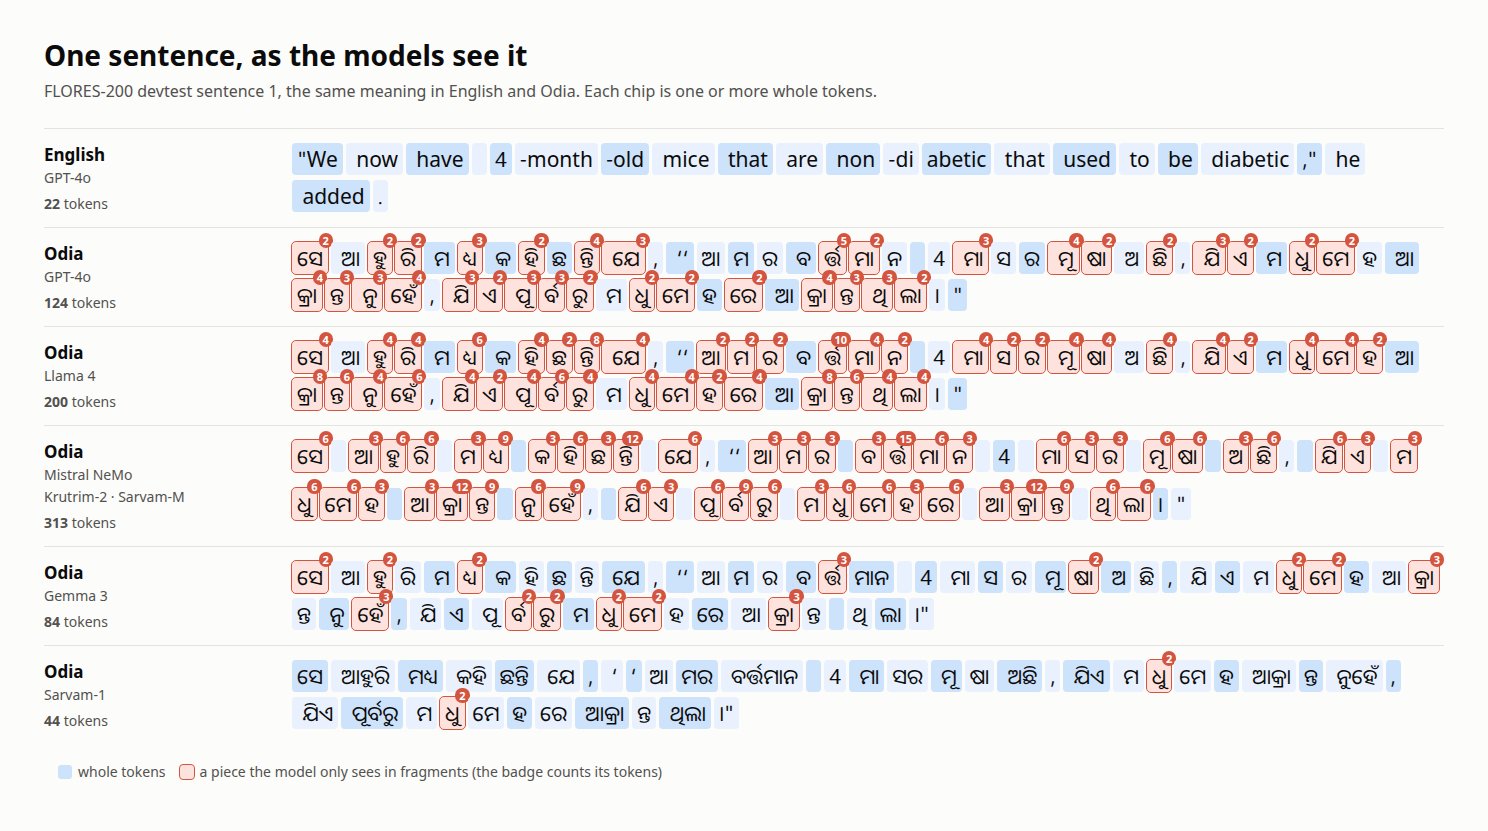
\includegraphics[width=\columnwidth]{figures/sentence.png}
\caption{One FLORES-200 sentence in English (GPT-4o) and in Odia on five tokenizers. Red boxes are
pieces the model sees only as byte fragments, with the number of tokens each takes; on Tekken almost
every Odia character is one.}
\label{fig:sentence}
\end{figure}

\paragraph{Tokenizers are inherited.} Krutrim-2's tokenizer file is byte-identical to Mistral NeMo's,
and Sarvam-M's gives identical token counts in every language we measured; both were built on
Mistral models. Their Odia tax (12.87\x) is the highest of any tokenizer we measured, and 2.6\x\ that of
GPT-4o.

\paragraph{The rest of the picture.} Weighted by speakers, Indian text costs 1.92\x\ English on
GPT-4o, 2.37\x\ on Llama~4, 4.80\x\ on Llama~3 and 5.28\x\ on Qwen. Odia is the most expensive major
language on almost every general-purpose tokenizer; Santali in Ol Chiki is the most expensive
language overall (13.70\x\ on GPT-4o, worse than GPT-4's 12.74\x). GPT-4o breaks 53\% of Odia
letters; on Llama~3, 99\% of the tokens produced for Odia are byte fragments. Indic-focused
tokenizers show the tax is not inherent to the scripts, but their coverage has limits: Sarvam-1, the
best measured for Odia among model tokenizers (1.46\x), costs 7.39\x\ for Urdu and 11.77\x\ for
Santali, outside the ten languages it was built for.

\section{Removing both causes from an existing tokenizer}
\label{sec:fix}

We extend Qwen~2.5's byte-level BPE tokenizer \citep{qwen2025qwen25} with two changes, chosen so that
a model trained with the original tokenizer keeps every token it knows.

\paragraph{Marks.} We modify the pre-tokenizer so that a word may continue over combining marks of
the Indic scripts only (the Unicode blocks from Devanagari to Sinhala, Ol Chiki and Meetei Mayek). Text without
these marks is cut exactly as before. Allowing every combining mark would also change Thai, for
reasons explained in \S\ref{sec:dead}.

\paragraph{Confined merges.} New merges are learned by continuing BPE from Qwen's own segmentation of
web text, and appended after Qwen's 151,387 merges. Every new merge is required to produce a token
that contains the UTF-8 bytes of a script in which Indian languages are written (the Brahmic blocks,
Ol Chiki, Meetei Mayek, and the Arabic block used for Urdu, Kashmiri and Sindhi). Text containing none
of those bytes cannot trigger a new merge and is encoded exactly as before. For lipi-Indic we learn merges on FineWeb-2
\citep{penedo2025fineweb2}: 12--18\,MB per language where available and all available text for
Awadhi, Santali, Magahi and Kashmiri (22.8 million words in all), with every document containing a
FLORES sentence removed. Capping the data per language keeps Hindi from taking most new tokens.

\paragraph{What changes, and what does not.} English, French, Spanish, Russian, Chinese, Japanese,
Korean, Thai and Hebrew receive exactly the same token ids as from Qwen~2.5. Arabic and Persian
change, because Urdu, Kashmiri and Sindhi share their script; both become cheaper (Arabic 1.63\x\ to
1.54\x, Persian 2.58\x\ to 1.79\x), but those tokens were learned on Urdu text.

\paragraph{Both changes are needed.} For Odia alone (Table~\ref{tab:ablation}), new tokens without
the marks change stop at the pre-tokenizer's floor (2.34\x\ with 16K tokens); the marks change without
new tokens does nothing, because the vocabulary contains no Odia words to use it with. Together, 16K
new tokens bring Odia from 9.70\x\ to 1.13\x\ English.

\begin{table}[t]
\centering
\small
\begin{tabular}{lrrrrr}
\toprule
& \multicolumn{5}{c}{Odia (\x\ English) with $N$ new tokens} \\
tokenizer & 0 & 1K & 4K & 16K & 32K \\
\midrule
as shipped & 9.70 & & & & \\
marks only & 9.70 & & & & \\
tokens only & & 2.53 & 2.38 & 2.34 & \\
both & & 1.98 & 1.44 & \textbf{1.13} & 1.04 \\
\bottomrule
\end{tabular}
\caption{Ablation for Odia on FLORES-200 devtest (held out from the merge-learning data).}
\label{tab:ablation}
\end{table}

\paragraph{lipi-Indic against GPT-4o and Gemini.} Table~\ref{tab:indic} and Figure~\ref{fig:indic}
compare lipi-Indic at several sizes. With 96K new tokens (247,665 in all, fewer than Gemma~3's
262,145), it takes fewer tokens than both GPT-4o's and Gemini's tokenizers in 23 of the 24 languages;
the exception is Bengali (1.25\x\ against Gemini's 1.21\x). The largest gains are where current
tokenizers are worst: Odia 1.35\x\ (GPT-4o 4.99\x, Gemini 3.51\x), Santali 1.52\x\ (13.70\x,
5.25\x), Manipuri 1.41\x\ (3.07\x, 2.51\x). Sarvam-1 remains better than lipi-Indic on the ten
languages it was built for, with a 68K vocabulary devoted almost entirely to them.

\begin{table}[t]
\centering
\small
\begin{tabular}{lrr}
\toprule
tokenizer & vocabulary & weighted tax \\
\midrule
Qwen 2.5 / 3 & 151,665 & 5.28\x \\
GPT-4o / GPT-5 & 200,019 & 1.92\x \\
Sarvam-1 & 68,096 & 1.60\x \\
Gemini (Gemma 3) & 262,145 & 1.58\x \\
lipi-Indic 16K & 167,665 & 1.74\x \\
lipi-Indic 32K & 183,665 & 1.54\x \\
lipi-Indic 64K & 215,665 & 1.38\x \\
\textbf{lipi-Indic 96K} & 247,665 & \textbf{1.30\x} \\
lipi-Indic 128K & 279,665 & 1.26\x \\
\bottomrule
\end{tabular}
\caption{Speaker-weighted token tax over the 24 Indian languages.}
\label{tab:indic}
\end{table}

\begin{figure}[t]
\centering
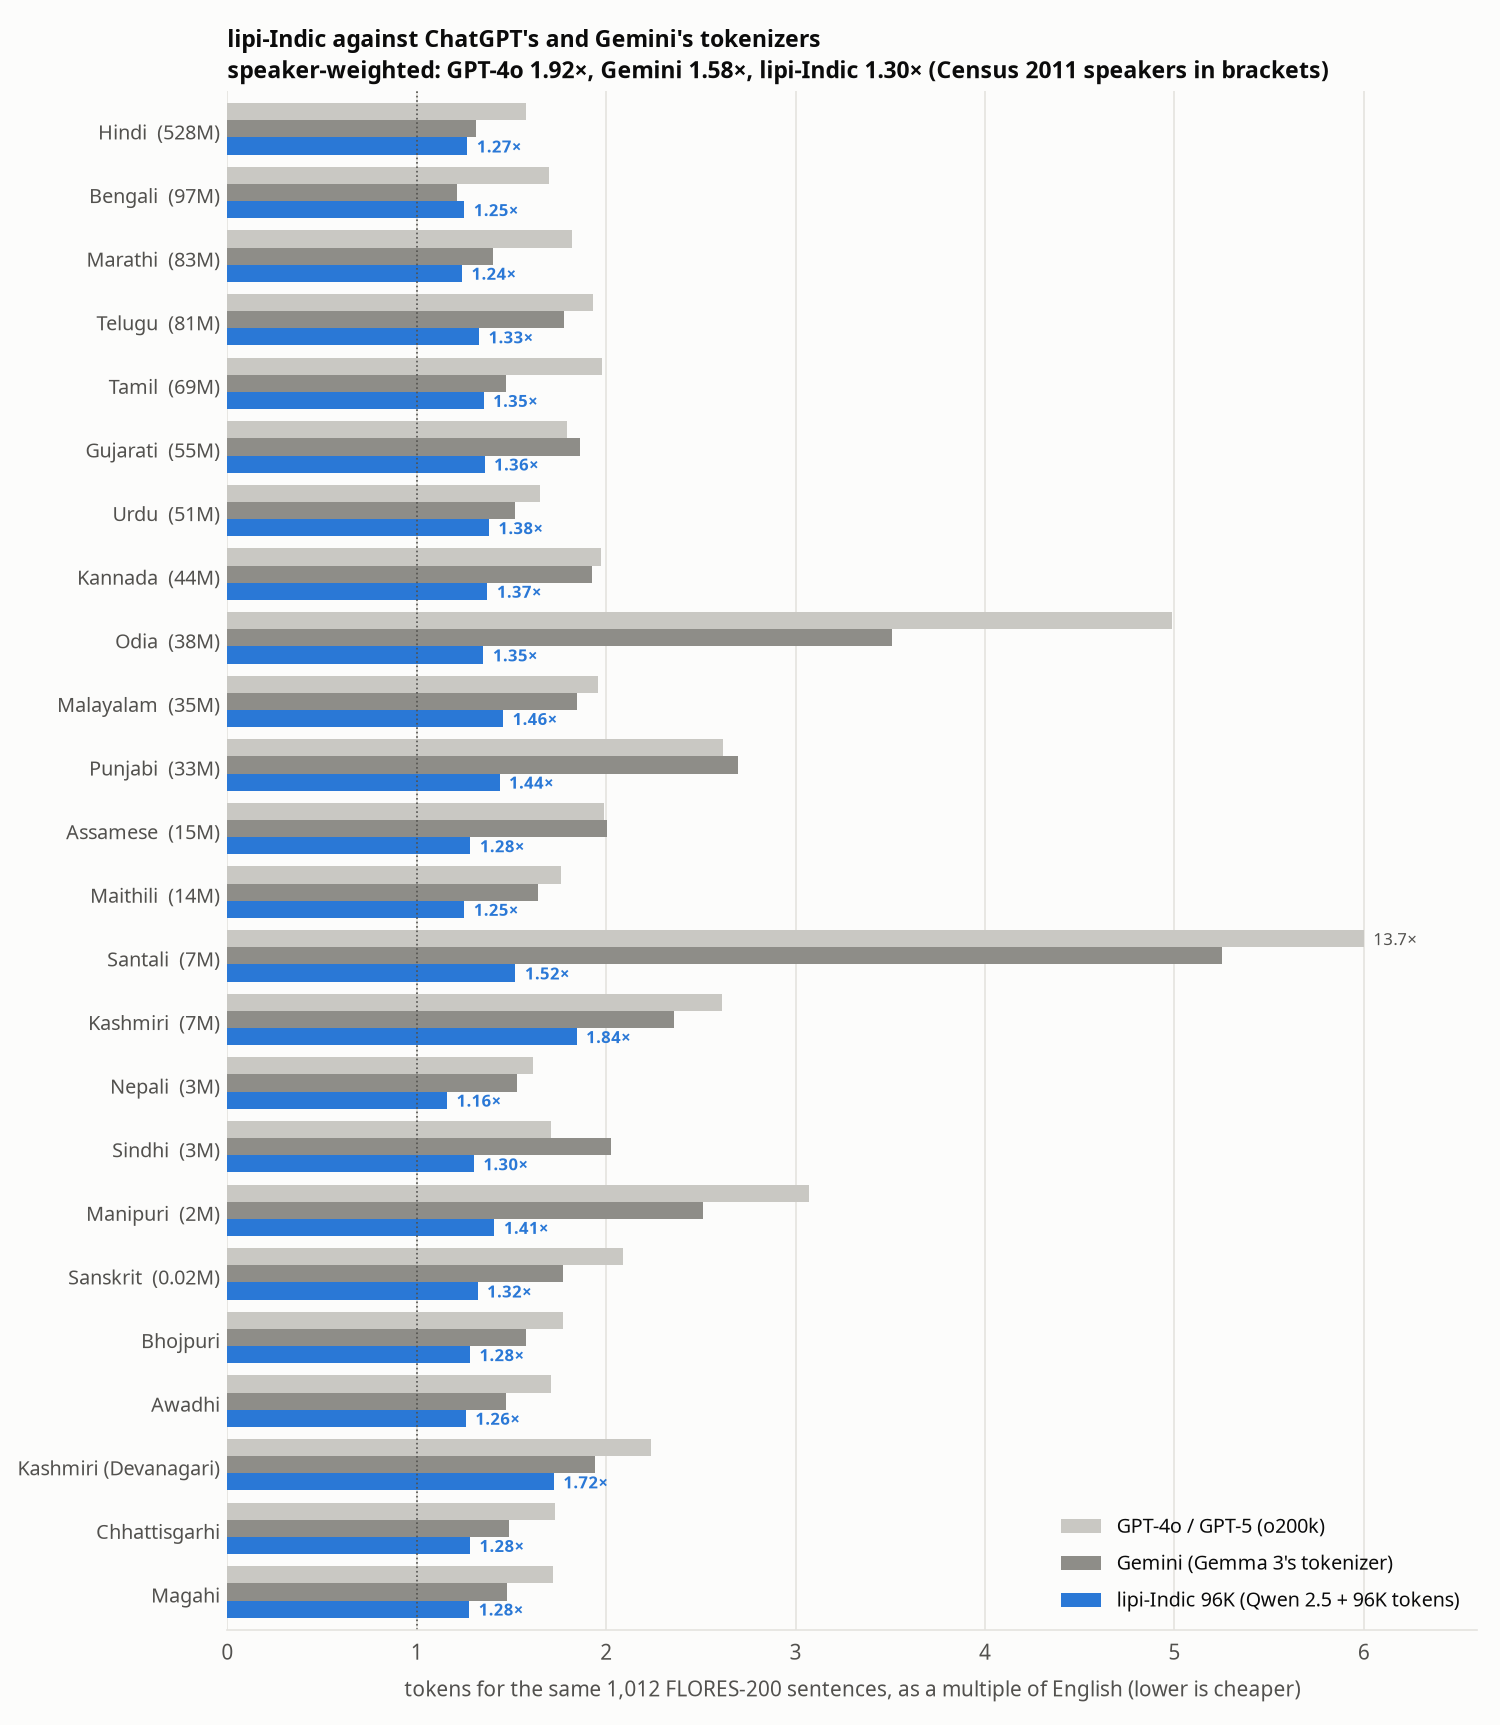
\includegraphics[width=\columnwidth]{figures/indic.png}
\caption{Token tax per language: lipi-Indic 96K against GPT-4o's and Gemini's tokenizers.}
\label{fig:indic}
\end{figure}

\section{Tokens the model was never shown}
\label{sec:dead}

Qwen~2.5's vocabulary contains 1,735 tokens that join a letter with a following combining mark. Since
its pre-tokenizer cuts before every mark, 1,667 of them can never be produced when encoding text. We
compare their input embeddings with the mean embedding: their cosine similarity to it is 0.94 on
average, against 0.38 for randomly chosen tokens, consistent with rows that received little or no
gradient during pre-training \citep{land2024magikarp}. A pre-tokenizer change that allowed every
combining mark would start producing these tokens, including for Thai, and send text through rows the
model never learned. lipi-Indic therefore relaxes the pre-tokenizer only for Indic marks.

\section{Training with the extended tokenizer}
\label{sec:model}

\paragraph{Setup.} We extend Qwen~2.5~0.5B with the 16K Odia tokenizer of Table~\ref{tab:ablation};
each new embedding row starts as the mean of the rows of the pieces it replaces
\citep{hewitt2021initializing}. We continue pre-training on Odia web text from FineWeb-2 plus a
quarter as much English, in three arms with all else equal: \textbf{A}, Qwen's own tokenizer on
24\,MB of Odia and 6\,MB of English (19.9M tokens); \textbf{B}, the extended tokenizer on the same
30\,MB (3.5M tokens); \textbf{C}, the extended tokenizer for as many tokens as A, which is the same
GPU time (135\,MB of Odia and 34\,MB of English). New embedding rows learn at $5\times10^{-4}$, all
other parameters at $5\times10^{-5}$; training uses data parallelism with optimizer-state sharding
on two NVIDIA T4 GPUs. We report bits per byte, which is comparable across tokenizers, on FLORES
devtest and on 500 held-out web documents; chrF++ \citep{popovic2017chrf} for five-shot translation
on 200 FLORES sentences; and Belebele \citep{bandarkar2024belebele} reading comprehension in Odia.

\begin{table*}[t]
\centering
\small
\resizebox{\textwidth}{!}{%
\begin{tabular}{lrrrrr}
\toprule
& Qwen 2.5 0.5B & extended, untrained & A (Qwen tok.) & B (ext., same text) & C (ext., same time) \\
\midrule
tokens for the Odia FLORES devtest & 267,893 & 31,211 & 267,893 & 31,211 & 31,211 \\
training time, 2\x\ T4 (min) & -- & -- & 104 & \textbf{19} & 108 \\
Odia bits/byte, FLORES devtest & 1.444 & 1.183 & 0.751 & 0.782 & \textbf{0.674} \\
Odia bits/byte, held-out web & 1.130 & 1.103 & 0.575 & 0.608 & \textbf{0.461} \\
English bits/byte, FLORES devtest & \textbf{1.076} & 1.205 & 1.164 & 1.106 & 1.127 \\
Odia$\to$English chrF++ & 16.0 & 11.3 & 0.0 & 15.4 & \textbf{24.8} \\
English$\to$Odia chrF++ & 8.7 & 2.6 & \textbf{10.8} & 3.7 & 8.3 \\
Belebele, Odia (accuracy, \%) & 30.6 & 23.0 & 29.2 & 31.3 & 30.1 \\
time to score Belebele, Odia (s) & 382 & 46 & 385 & \textbf{46} & \textbf{44} \\
\bottomrule
\end{tabular}}
\caption{Continued pre-training of Qwen~2.5~0.5B with its own tokenizer (A) and the Odia-extended
tokenizer (B, C). One run per arm.}
\label{tab:model}
\end{table*}

\paragraph{Results.} Table~\ref{tab:model} and Figure~\ref{fig:m1}. \emph{Same text}: B reads A's
30\,MB in 19 minutes instead of 104 (5.4\x\ less compute) and ends within 4\% of A's bits per byte
on FLORES (6\% on web text), while losing less English (+2.8\% bits per byte against A's +8.2\%).
\emph{Same compute}: in A's time, C reads 5.6\x\ as much Odia and reaches 10\% lower bits per byte on
FLORES and 20\% on held-out web text. \emph{Initialisation}: without any training, the extended
model already predicts Odia better than the original (1.183 against 1.444 bits per byte).
\emph{Inference}: scoring Belebele in Odia takes 46\,s instead of 382\,s.

\paragraph{Results against the fix.} Belebele does not separate the arms: every model scores
23--31\% (chance is 25\%; one standard error is 1.5 points), so a 0.5B model cannot do this task in
Odia either way. English$\to$Odia translation is worse with the extended tokenizer (B 3.7, C 8.3
against A's 10.8): in the samples we inspected, the extended models copy the English sentence back
instead of translating. A's Odia$\to$English translations score near zero; this run kept only five
outputs per model, so the cause is not established (evaluations now keep every output). English
bits per byte worsen in every arm (+2.8\% to +8.2\%) despite 20\% English in the mix.

\begin{figure}[t]
\centering
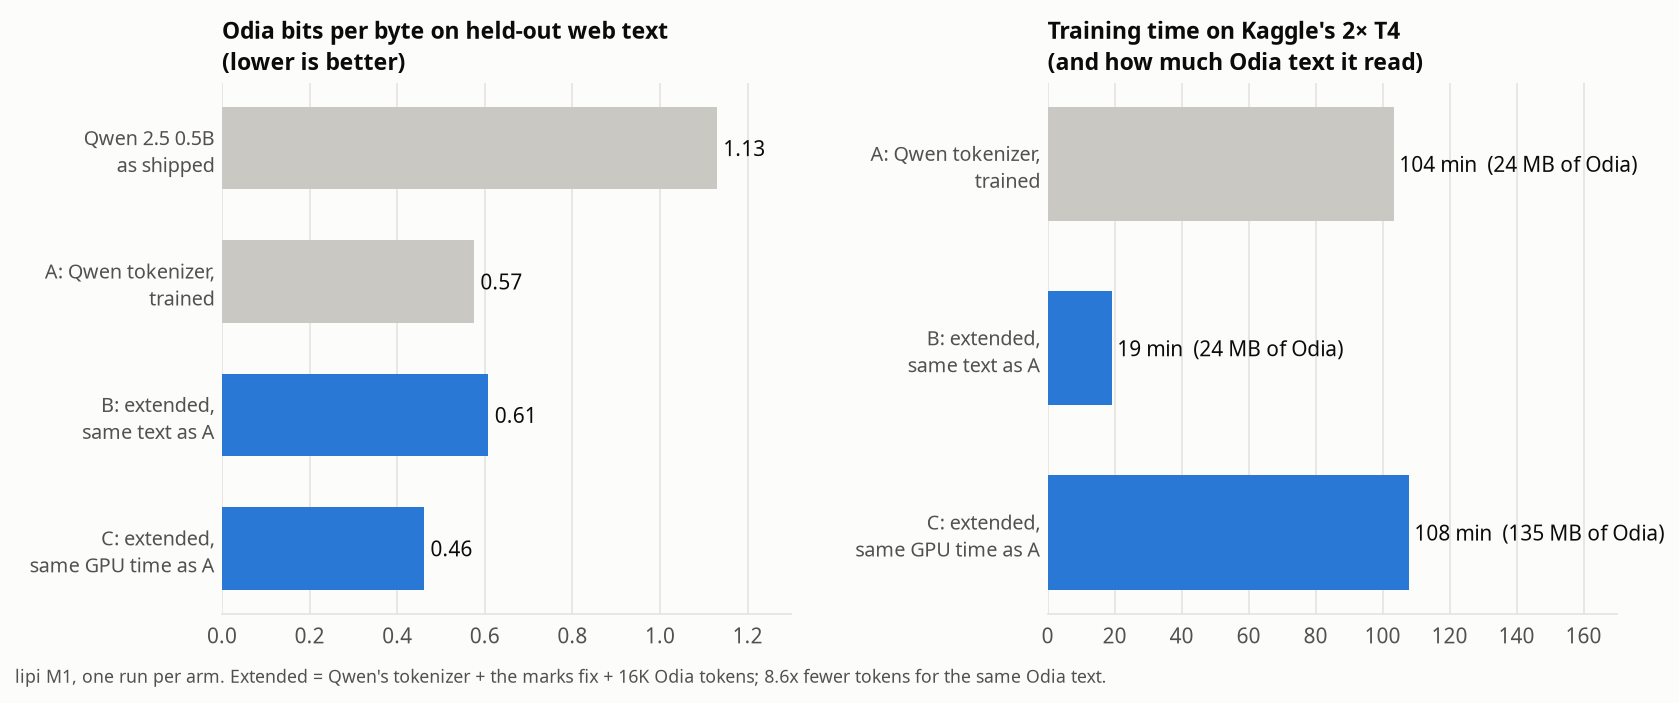
\includegraphics[width=\columnwidth]{figures/m1.png}
\caption{Odia bits per byte on held-out web text (left) and training time on two T4 GPUs (right), per arm.}
\label{fig:m1}
\end{figure}

\section{What the token tax costs in time}
\label{sec:speed}

Token counts become latency: a model writes one token per step. On one T4 in fp16, we time
Qwen~2.5~0.5B writing 40 FLORES devtest sentences per language, forced to the reference text so that
every tokenizer writes exactly the same words, at batch sizes 1 and 16. Speed per step does not
depend on the trained weights, so the extended models are used untrained.

\begin{table}[t]
\centering
\small
\begin{tabular}{lrrr}
\toprule
language & Qwen & lipi-Indic & speed-up \\
\midrule
English & 0.83 & 0.84 & 0.99\x \\
Hindi & 3.73 & 1.12 & 3.3\x \\
Bengali & 4.33 & 1.08 & 4.0\x \\
Tamil & 5.28 & 1.17 & 4.5\x \\
Telugu & 5.89 & 1.13 & 5.2\x \\
Odia & 8.37 & 1.19 & 7.0\x \\
Urdu & 2.71 & 1.20 & 2.3\x \\
Santali & 6.91 & 1.28 & 5.4\x \\
\bottomrule
\end{tabular}
\caption{Seconds to write one FLORES sentence with each tokenizer, batch 1, Qwen~2.5~0.5B on one T4.}
\label{tab:speed}
\end{table}

Each step costs the same with either tokenizer (26.4--27.4\,ms), so the larger vocabulary does not
slow the model; what changes is the number of steps (Table~\ref{tab:speed}). With Qwen's tokenizer an
Odia sentence takes 10\x\ as long to write as an English one; with lipi-Indic, 1.4\x. Batch size 16
gives the same picture (2.2--6.7\x). For reading, the 3,000-character Odia document that takes 5,923
tokens and 3.40\,s to prefill with Qwen's tokenizer takes 650 tokens and 0.088\,s with lipi-Indic
(39\x) and 618 tokens and 0.068\,s with the Odia-only tokenizer (50\x); prefill time grows faster
than linearly with length, so the time saved exceeds the tokens saved. In a 32K-token context,
lipi-Indic fits 881 FLORES Odia sentences instead of 116.

\section{Discussion}

The pre-tokenization bound of \citet{regmi2026vowel} gives practitioners a quick test: if a
tokenizer's floor for a script is well above 1\x\ English, vocabulary work alone cannot fix it, and
the pre-tokenizer must change first. Because the
measurement needs only the tokenizer and parallel text, it can be run on any new model before
release. The confined extension shows that both causes can be removed from an existing open model
without disturbing what it knows of other languages, at a vocabulary size below Gemini's.

\section*{Limitations}

The model results come from one run per arm with a 0.5B model and short continued pre-training;
differences of a few percent are within what another seed could change, and larger models may behave
differently. We trained a model only on the Odia tokenizer; training on lipi-Indic needs text in all
24 languages and is future work. FLORES-200 is formal, translated news and travel text;
conversational, code-mixed or romanised text will be taxed differently. Bodo, Dogri and Konkani are
missing from FLORES-200. Gemini's tokenizer is approximated by Gemma~3's and not verified against
Google's token counting. Token counts are not prices: providers set their own prices per token. The
speed measurements use forced decoding of reference sentences on one GPU and model size.

\section*{Ethics statement}

FLORES-200 is released under CC BY-SA 4.0 and FineWeb-2 under the ODC-By licence; we use them as
intended for research. The work aims to reduce a cost borne disproportionately by speakers of
lower-resourced Indian languages.

\section*{Use of AI assistants}

AI coding and writing assistants were used to help write code and prose. The author designed the
study, checked every reported number against the released scripts and outputs, and takes
responsibility for the content.

\bibliography{refs}

\end{document}
